\documentclass[11pt]{article}
\usepackage[margin=1in]{geometry}
\usepackage{graphicx}
\usepackage{booktabs}
\usepackage{amsmath,amssymb}
\usepackage{xcolor}
\usepackage[colorlinks=true,linkcolor=blue!50!black,urlcolor=blue!50!black]{hyperref}
\graphicspath{{../figures/}}

\title{\textbf{Quaternion--Phase Pooling for Rotation-Invariant Vision}\\[2pt]
\large A Nagare closed-form study: from a failed rotor-pool to a domain-tunable phase descriptor}
\author{Aiko (agent) for Cs.\ Hajdu \\ \small Nagare (\texttt{nagare-holonomy-learn}), closed-form Rust, no autograd}
\date{2026-07-10}

\begin{document}
\maketitle

\begin{abstract}
We study rotation-invariant image classification with closed-form (no-autograd) models built on
signed-hypergraph and Clifford-rotor primitives. A na\"ive \emph{rotor pool}---rotating learned
feature channels by a quaternion---fails, because those channels are not rotation-equivariant and
the rotation scrambles them. The fix is to pool the rotor's \emph{phase} (the gradient orientation,
$e^{i\theta}$, a unit $z$-quaternion) rather than a rotated vector: the resulting orientation
histogram \emph{circularly shifts} under image rotation, so its $|\mathrm{DFT}|$ is an
\emph{exact} rotation invariant. This phase-pool wins decisively on synthetic shapes ($0.97$ vs
$0.52$--$0.65$ for every alternative), generalises to a dihedral-equivariant hypergraph convolution
(proven), and---on real data---exhibits a clean \emph{rank flip}: worst on upright MNIST digits
($0.42$), best on KTH-TIPS textures ($0.61$). A \emph{spatial phase map} (an $R\times R$ grid of
local phase descriptors) fuses locality and phase-invariance in one descriptor, tuning the
invariance$\leftrightarrow$locality trade by $R$: it lifts MNIST from $0.42$ to $0.88$ while $R{=}1$
(global) remains optimal for textures. Everything is closed-form, dependency-free, and reproducible.
\end{abstract}

\section{Motivation}
Nagare is a closed-form machine-learning substrate (forward/backward operator pairs over flat
buffers, no autograd tape) targeting signed hypergraphs and Clifford algebra. Its flagship result is
signed-graph link prediction; this report is the \emph{computer-vision expansion}. The question:
can the framework's Clifford-rotor and entropy primitives buy rotation-invariance the ``right''
way---by construction, not by data augmentation?

\section{The rotor pool fails; pool the phase instead}
The intuitive move is a \emph{rotor pool}: represent each patch by a learned feature vector, rotate
it by a (free or geometric) quaternion, aggregate. Measured on randomly-rotated synthetic shapes,
every version \emph{hurts} or ties a plain mean-pool (Table~\ref{tab:ladder}). The mechanism, isolated:
a learned patch embedding is \emph{not} rotation-equivariant---it does not co-rotate with the
image---so rotating it is noise, not canonicalisation.

The correction (due to Hajdu) is to pool the rotor's \emph{phase}, not a rotated vector. Each pixel's
gradient orientation $\theta=\operatorname{atan2}(\partial_y,\partial_x)$ is a genuine geometric
phase ($e^{i\theta}$, a unit $z$-quaternion). Magnitude-weighted pooling of these phases is an
orientation histogram $h$. Under a global image rotation $\varphi$, every $\theta\!\to\!\theta+\varphi$,
so $h$ \emph{circularly shifts}. Therefore
\[
  |\mathrm{DFT}(h)|_k \quad\text{is an \emph{exact} rotation invariant of the whole orientation distribution,}
\]
losing nothing to rotation while keeping all discriminative orientation structure. No feature vector
is ever rotated---only phases are pooled.

\begin{table}[t]
\centering
\caption{Rotation-invariant shape ID (synthetic, median over 4 seeds). Pooling the \emph{phase}
crushes every rotate-the-vector or canonicalise approach.}
\label{tab:ladder}
\begin{tabular}{lc}
\toprule
approach & median accuracy \\
\midrule
vector rotor-pool (learned, on channels) & 0.52 \emph{(fails)} \\
single-$\theta$ canonicalisation & 0.60 \\
$C_8$ group-convolution & 0.65 \\
raw orientation histogram (covariant) & 0.61 \\
\textbf{phase-pool} $|\mathrm{DFT}|$ & \textbf{0.97} \\
\bottomrule
\end{tabular}
\end{table}

\begin{figure}[t]
\centering
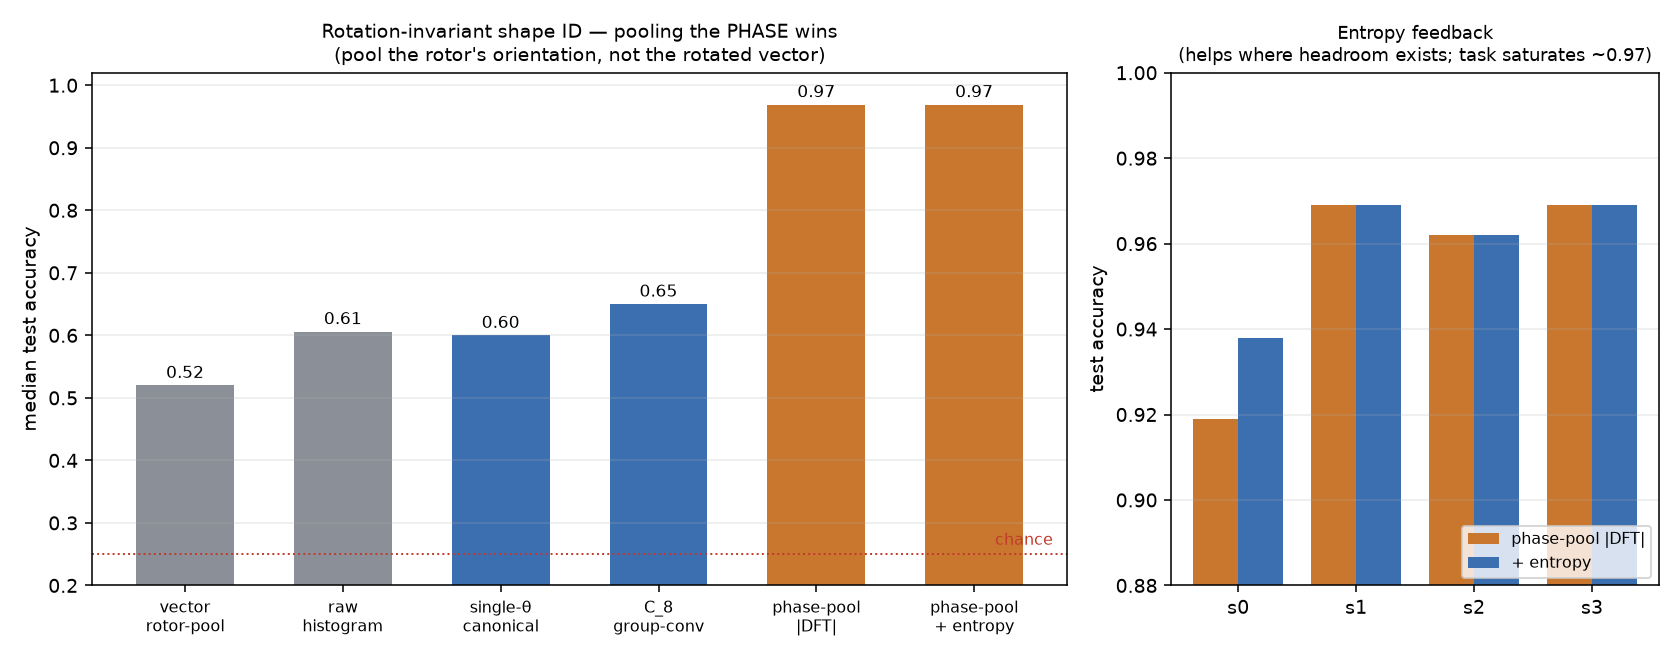
\includegraphics[width=0.92\linewidth]{phase-pool-cv-ladder.png}
\caption{The approach ladder on rotation-invariant shape ID. Pooling the phase (orange) dominates
every earlier approach by $\ge 0.3$; entropy as a feature is neutral once $|\mathrm{DFT}|$ saturates.}
\label{fig:ladder}
\end{figure}

\section{Dihedral-equivariant hypergraph convolution}
The single continuous canonicalisation is the $n\!\to\!\infty$ / single-frame case of a finite
\emph{dihedral group} $D_n$. Steering the geometric messages of the signed hypergraph convolution
across $D_n$ yields a group-equivariant operator; we \emph{prove} (unit tests, $|\Delta|<10^{-5}$)
that the node$\to$edge and edge$\to$node message passes commute with the group action and the
group-pool is $D_n$-invariant. Empirically a learned $C_8$ group-convolution edges out the
single-frame canonicalisation ($0.65$ vs $0.60$) at $8\times$ compute---but the phase-pool
$|\mathrm{DFT}|$ ($0.97$) is far stronger still, because it is the \emph{exact} invariant of the
\emph{entire} orientation distribution rather than a discrete-group average.

\emph{Entropy.} We tested phase entropy $H(h)=-\sum p\log p$ both as a feature and as a
spectral-entropy regulariser on a learned feature map. It is neutral-to-slightly-harmful for
supervised classification: as a feature it is redundant with $|\mathrm{DFT}|$ (both shift-invariant
histogram summaries); as a spread prior it fights the low-entropy concentration supervised
discrimination wants. Its home is un/self-supervised, collapse-prone objectives.

\section{Real datasets: the rank flip}
On real data (MNIST digits, KTH-TIPS textures; models trained upright, evaluated upright and on
randomly-rotated test) the same descriptor gives \emph{opposite} outcomes (Table~\ref{tab:real},
Fig.~\ref{fig:datasets}). The phase-pool is \emph{worst} on digits and \emph{best} on textures.

\begin{table}[t]
\centering
\caption{Real datasets, upright / rotated test accuracy. Phase-pool: worst on digits (spatial,
canonical pose), best on textures (rotation-nuisance, orientation-driven).}
\label{tab:real}
\begin{tabular}{llcc}
\toprule
dataset & arm & upright & rotated \\
\midrule
MNIST (digits) & raw-pixel linear & 0.881 & 0.249 \\
 & patch-embed (spatial) & 0.855 & 0.266 \\
 & phase-pool $|\mathrm{DFT}|$ & \textbf{0.416}\,$\leftarrow$ worst & 0.287 \\
\midrule
KTH-TIPS (textures) & raw-pixel linear & 0.512 & 0.310 \\
 & patch-embed (spatial) & 0.429 & 0.325 \\
 & phase-pool $|\mathrm{DFT}|$ & \textbf{0.606}\,$\leftarrow$ best & \textbf{0.458}\,$\leftarrow$ best \\
\bottomrule
\end{tabular}
\end{table}

Digit identity needs \emph{spatial layout} and a \emph{canonical pose}, both of which the phase-pool
discards; texture identity is \emph{orientation-statistics driven} and \emph{pose-free}, the
phase-pool's exact strength. Textures are moreover \emph{genuinely} rotation-invariant (a rotated
brick is a brick), with no $6\!\leftrightarrow\!9$ ambiguity ceiling, so the invariance is a pure
asset: the phase-pool is best both upright and rotated on KTH-TIPS.

\begin{figure}[t]
\centering
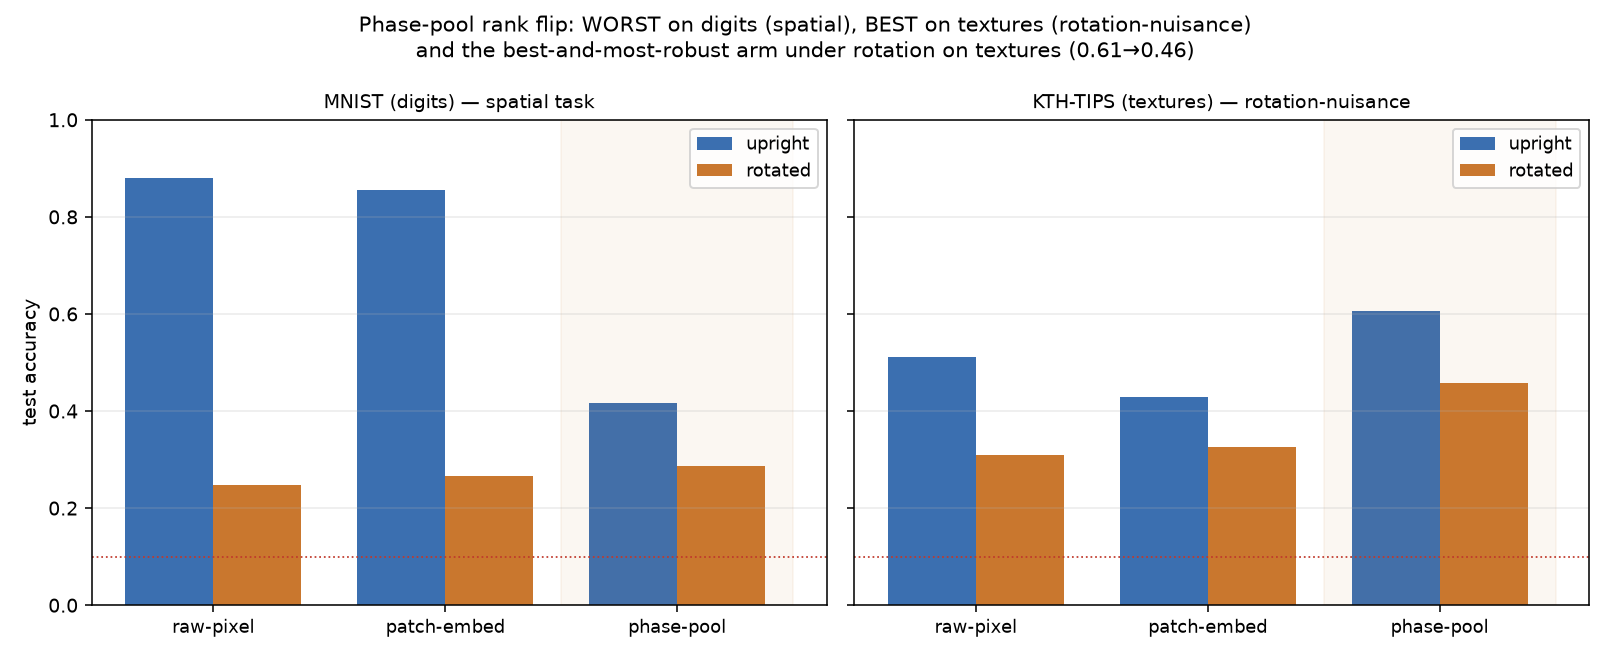
\includegraphics[width=\linewidth]{cv-datasets-phase-pool.png}
\caption{The rank flip. Phase-pool (rightmost group) is worst on MNIST digits, best on KTH-TIPS
textures; upright vs randomly-rotated test.}
\label{fig:datasets}
\end{figure}

\section{The spatial phase map: locality $\times$ phase, tuned by $R$}
The $R\times R$ \emph{spatial phase map} computes one orientation-$|\mathrm{DFT}|$ per grid cell and
concatenates. $R{=}1$ is the global phase-pool (full invariance, no layout); larger $R$ keeps coarse
layout (each cell locally rotation-invariant, but the cell \emph{arrangement} is not). Sweeping $R$
traces the invariance$\leftrightarrow$locality trade, and its optimum is \emph{domain-dependent}
(Table~\ref{tab:sweep}, Fig.~\ref{fig:ablation}): locality lifts MNIST from $0.42$ to $\mathbf{0.88}$
(the best arm, beating raw pixels), while $R{=}1$ (global) is optimal for textures.

\begin{table}[t]
\centering
\caption{Spatial phase map $R$-sweep, upright accuracy (train-upright). Opposite trends: locality
lifts digits, global is best for textures.}
\label{tab:sweep}
\begin{tabular}{lcc}
\toprule
$R$ (grid) & MNIST & KTH-TIPS \\
\midrule
1 (global phase-pool) & 0.416 & \textbf{0.606} \\
2 & 0.763 & 0.601 \\
4 & 0.856 & 0.567 \\
7 / 8 & \textbf{0.884} & 0.512 \\
\bottomrule
\end{tabular}
\end{table}

A cross-model \emph{mix} (pixels $\oplus$ phase) is best upright on MNIST ($0.898$) but collapses
under rotation ($0.266$) when trained upright---it leans on the dominant spatial path. Rotation
augmentation flattens every drop to $\approx 0$ (at an upright cost); the best rotation-robust arm is
the \emph{domain-matched spatial phase map} (MNIST $R{=}7$: $0.60$; KTH $R{=}2$: $0.58$), beating the
crude concat. The spatial phase map is thus the genuine ``mixing for lifting'': it fuses locality and
per-cell phase-invariance in \emph{one} descriptor, with $R$ as a clean domain knob.

\begin{figure}[t]
\centering
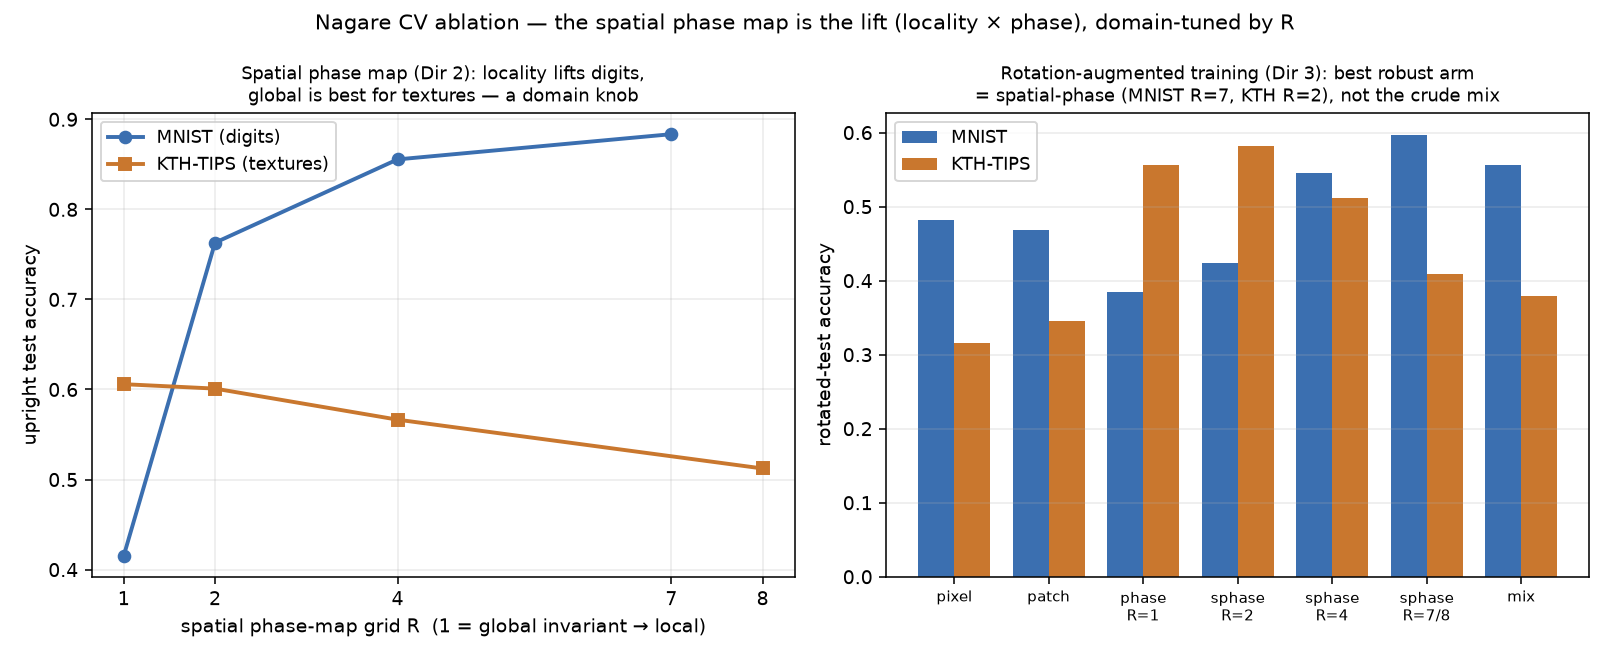
\includegraphics[width=\linewidth]{cv-ablation-sweep.png}
\caption{Left: the $R$-sweep---locality lifts digits, hurts textures (a domain knob). Right:
rotation-augmented training makes every arm rotation-robust; the best robust arm is the
domain-matched spatial phase map, not the crude mix.}
\label{fig:ablation}
\end{figure}

\section{Conclusions}
Pooling the quaternion \emph{phase}---not a rotated feature vector---delivers exact
rotation-invariance and is the strongest closed-form descriptor by a wide margin on the tasks it
suits (orientation-driven, rotation-nuisance textures). It generalises to a proven
dihedral-equivariant hypergraph convolution. Its scope is characterised on two real datasets (the
rank flip), and the spatial phase map lifts it onto layout-dependent tasks with $R$ as the domain
knob. Recommended deployment: ship the phase machinery with $R$ documented---$R{=}1$ for
rotation-nuisance tasks, high $R$ for layout tasks. Open: a \emph{native-rotation} texture benchmark
(KTH-TIPS2 / Kylberg-rotated) to measure clean invariance without self-imposed rotation artifacts.

\vspace{6pt}
\noindent\small\textbf{Reproducibility.} All results are closed-form, seeded, dependency-free
(no image crate; PIL decodes PNGs to raw bytes off-line). Code: \texttt{src/vision.rs},
\texttt{examples/cv\_bench.rs}; data \texttt{\textasciitilde/nagare\_data/}. Run
\texttt{cargo run --release --example cv\_bench -- --dataset \{mnist|raw\} --data <dir> [--augment]}.

\end{document}
